\documentclass[11pt]{article} % For LaTeX2e
\usepackage{nips12submit_e,times}
%\documentstyle[nips12submit_09,times,art10]{article} % For LaTeX 2.09

%\usepackage[usenames,dvipsnames]{color}

\usepackage[utf8]{inputenc}
\usepackage[T1]{fontenc}
\usepackage{textcomp}
\usepackage[scaled=0.8]{beramono}

\usepackage{caption}
\usepackage{subcaption}
\usepackage{wrapfig}
\usepackage{amsmath,amssymb}
\usepackage{array}
\usepackage{tabularx}
\usepackage{booktabs}
\usepackage{graphicx}

\usepackage{cite}
\usepackage{url}
\usepackage[hyperfootnotes=false,citecolor=RedOrange,linkcolor=RoyalBlue,urlcolor=DarkOrchid,colorlinks]{hyperref}
\usepackage[all]{hypcap}

\newcommand{\todo}[1]{\noindent\texttt{\color[rgb]{0.5,0.1,0.1} TODO: #1}}


\newcommand{\sectref}[1]{\hyperref[#1]{\mbox{Section~\ref*{#1}}}}
\newcommand{\figref}[1]{\hyperref[#1]{\mbox{Figure~\ref*{#1}}}}
\newcommand{\tabref}[1]{\hyperref[#1]{\mbox{Table~\ref*{#1}}}}
\newcommand{\eqtref}[1]{\hyperref[#1]{\mbox{Equation~\ref*{#1}}}}

\newcommand{\argmax}{\operatornamewithlimits{argmax}}
\newcommand{\argmin}{\operatornamewithlimits{argmin}}
\newcommand{\twopartdef}[4]
{
	\left\{
		\begin{array}{ll}
			#1 & \mbox{if } #2 \\
			#3 & \mbox{if } #4
		\end{array}
	\right.
}

\title{Active Learning of Function Contours using Gaussian Process Confidence Bounds\thanks{Final
report for the course \emph{Research in Computer Science} (Spring
Semester 2012), carried out under the supervision of \emph{Prof. Andreas Krause.}}}

\author{
Alkis Gkotovos\\
Department of Computer Science, ETH Zurich\\
\texttt{alkisg@student.ethz.ch}
}

\nipsfinalcopy % Uncomment for camera-ready version

\begin{document}

\maketitle

\begin{abstract}
We present a novel heuristic for actively identifying function
contours using the framework of Gaussian processes to model the underlying
function and utilizing the
inferred confidence bounds to guide the learning process. We also show how
he proposed heuristic can be extended to identify $\epsilon$-optimal function
contours. Our method is evaluated and compared to the state of the art on
synthetic and real-world seismographic data.
\end{abstract}

\section{Introduction}


\section{Algorithm}
The problem of actively learning function contours can be described as follows.
Let ${f : \mathcal{D} \to \mathbb{R}}$ be the target function, where
$\mathcal{D}$ is a bounded subset of $\mathbb{R}^n$. We are interested in
finding the subset of $\mathcal{D}$ where this function takes values greater
than a specified threshold $t$, i.e. the set
$\mathcal{G}_t = \{x \in \mathcal{D} \mid f(x) > t\}$. To this end, we take
consecutive measurements $(x^{(i)}, f(x^{(i)}))$ of the function
and use them to determine $\mathcal{G}_t$. After the $i$-th step, the set of
all acquired measurements is
$\mathcal{M}^{(i)} = \{(x^{(1)}, f(x^{(1)})),\ldots,(x^{(i)}, f(x^{(i)}))\}$.

Our basic premise is that the time required to obtain each measurement is
non-negligible and, therefore, taking a large number of random measurements
over the whole domain $\mathcal{D}$ is prohibitive. We rather aim at directing
the measurement process so that the chosen points $x^{(i)}$ are informative with
respect to the desired contours, which should result in accurately determining
the set $\mathcal{G}_t$ using a significantly smaller number of measurements
compared to random sampling.

In this setting, we have to decide on (1) a model that allows us to use the
measurements in order to obtain an approximation of $\mathcal{G}_t$, and (2) a
strategy to select the next point of measurement at each step. The following
subsections deal with these two issues.

\subsection{Gaussian processes}
We chose to use Gaussian processes~\cite{gpbook} in modeling the target
function $f$, as they have been successfully used before in the context of
contour detection~\cite{bryan2005, bryan2008}. Gaussian process regression
offers a non-parametric framework for predicting the values of the function at
unobserved points, given a number of measurements. The characteristics of
the assumed underlying model are primarily specified by a kernel function
${K : \mathcal{D} \times \mathcal{D} \to \mathbb{R}}$, which determines the
covariance of any two points in $\mathcal{D}$.

In our active learning setting, $\mathcal{M}^{(i)}$ is used as a training set
for Gaussian process regression and the inferred mean $m^{(i)}(x)$ of the
model is used to approximate the set $\mathcal{G}_t$ as
${\mathcal{G}^{(i)}_t = \{x \in \mathcal{D} \mid m^{(i)}(x) > h\}}$.

\subsection{Choosing the next point}
The general strategy for choosing the next point of measurement at each step $i$
is to first establish a finite set $\mathcal{C}^{(i)} \subseteq \mathcal{D}$ of
candidate points, then evaluate some heuristic
${h : \mathcal{C}^{(i)} \to \mathbb{R}}$ for each candidate point and, finally,
choose the point with the largest heuristic value, that is
\begin{align*}
  x^{(i+1)} = \underset{x \in \mathcal{C}^{(i)}}{\argmax}\{h(x)\}
\end{align*}
If $\mathcal{D}$ is finite, we can use
$\mathcal{C}^{(i)} = \mathcal{D}\setminus\mathcal{M}_i$ or a random subset
thereof in case $\mathcal{C}_i$ is too large. Otherwise, we have to sample a set
of candidate points from $\mathcal{D}$. Random sampling is preferred over a
fixed grid to get better coverage of $\mathcal{D}$~\cite{bryan2005}.

Choosing the heuristic $h$ involves an exploration-exploitation trade-off. The
state of the art in contour detection combines the inferred variance of the
Gaussian process with the
distance from the inferred contour to create the straddle~\cite{bryan2005}
heuristic ${h_{straddle}(x) = 1.96\sigma(x) - | m(x) - t |}$, where $m(x)$
and $\sigma(x)$ are respectively the inferred mean and variance of the Gaussian
process at the candidate point $x$.

\begin{figure}[tb]
  \centering
  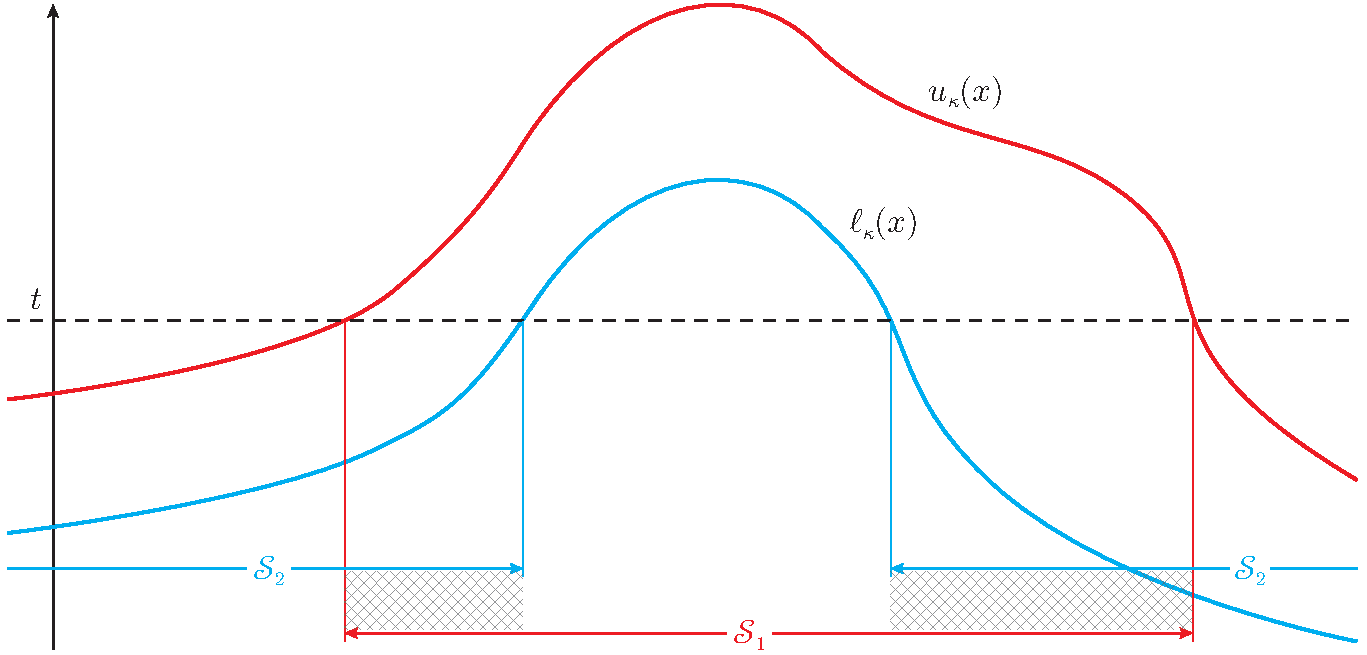
\includegraphics[width=\textwidth]{figures/cb}
  \caption{A one-dimensional example showing the two sets $\mathcal{S}_1$ and
           $\mathcal{S}_2$ and the
           the (shaded) confidence region
           $\mathcal{S} = \mathcal{S}_1\cap\mathcal{S}_2$.}
  \label{fig:cb}
\end{figure}

Our proposed heuristic is based on the fact that we can construct confidence
bounds for the desired contour by using the inferred mean and variance of
the Gaussian process. In particular, for every $x \in \mathcal{D}$ we obtain
a confidence interval ${[m(x) - \kappa\sigma(x), m(x) + \kappa\sigma(x)]}$,
where the probability of $x$ being in the interval depends on the value
of $\kappa$. Extending this idea and defining the functions
$u_{\kappa}(x) = m(x) + \kappa\sigma(x)$ and
$\ell_{\kappa}(x) = m(x) - \kappa\sigma(x)$,
we can create a confidence region for
the desired contour at level $t$ by using two sets
\begin{align*}
  \mathcal{S}_1 &= \{x \in \mathcal{D} \mid u_{\kappa}(x) \geq t\}\\
  \text{and}\hspace{1em}
  \mathcal{S}_2 &= \{x \in \mathcal{D} \mid \ell_{\kappa}(x) \leq t\}
\end{align*}
The confidence region is then
$\mathcal{S} = \mathcal{S}_1\cap\mathcal{S}_2$ (see~\figref{fig:cb}) and our
heuristic is defined
so that the point with the largest variance among the candidate points that
lie inside the confidence region is chosen:
\begin{align}\label{eq:hcb}
  h_{cb}(x) = \twopartdef { \sigma(x) } {x \in \mathcal{S}} {-\infty} {x \notin \mathcal{S}}
\end{align}
In other words, we exlude candidate points in the region where
$f(x) < t$ with high probability (the set $\mathcal{D}\setminus\mathcal{S}_1$)
and in the region where $f(x) > t$ with high probability
(the set $\mathcal{D}\setminus\mathcal{S}_2$).

From the above definitions it follows that 
$\mathcal{D}\setminus\mathcal{S}_2\subseteq\mathcal{S}_1$
and, equivalently, $\mathcal{S}\neq\varnothing$. We can also see that
obtaining more measurements leads to lower variance values, which in turn
generally reduces the size of $\mathcal{S}$.

\subsection{Identifying $\epsilon$-optimal contours}
The confidence bound heuristic described in the previous subsection can be
readily extended for detecting $\epsilon$-optimal function contours,
i.e. for approximating the set
${\mathcal{G}_{\epsilon} = \{x \in \mathcal{D} \mid f(x) > \underset{x \in \mathcal{D}}{\max}\,f(x) - \epsilon\}}$.
In this case, the sets used to define the confidence region $\mathcal{S}$
are defined as
\begin{align*}
  \mathcal{S}_1 &= \{x \in \mathcal{D} \mid u_{\kappa}(x) \geq \underset{x \in \mathcal{D}}{\max}\,\ell_{\kappa}(x) - \epsilon\}\\
  \text{and}\hspace{1em}
  \mathcal{S}_2 &= \{x \in \mathcal{D} \mid \ell_{\kappa}(x) \leq \underset{x \in \mathcal{D}}{\max}\,u_{\kappa}(x) - \epsilon\}
\end{align*}
Using the same confidence region $\mathcal{S} = \mathcal{S}_1\cap\mathcal{S}_2$
as before, runs the risk of exluding areas where the true maximum might lie.
Since the approximation
${\mathcal{G}^{(i)}_\epsilon = \{x \in \mathcal{D} \mid m^{(i)}(x) > \underset{x \in \mathcal{D}}{\max}\,m^{(i)}(x) - \epsilon\}}$
of $\mathcal{G}_{\epsilon}$ at each step
depends on the inferred maximum, it is important to have an accurate estimate
of the true maximum in order to get an accurate approximation of the desired
$\epsilon$-optimal contour. For that reason, we include in $\mathcal{S}$ the
region where the true maximum could still lie with high probability, i.e.
the set
\begin{align*}
  \mathcal{S}_3 &= \{x \in \mathcal{D} \mid u_{\kappa}(x) \geq \underset{x \in \mathcal{D}}{\max}\,\ell_{\kappa}(x)\}
\end{align*}
Therefore, the resulting confidence region is
$\mathcal{S} = \mathcal{S}_1\cap\mathcal{S}_2\cup\mathcal{S}_3$, as shown
in~\figref{fig:cbe}, and the heuristic function is the same as
in~\eqtref{eq:hcb}.

\begin{figure}[tb]
  \centering
  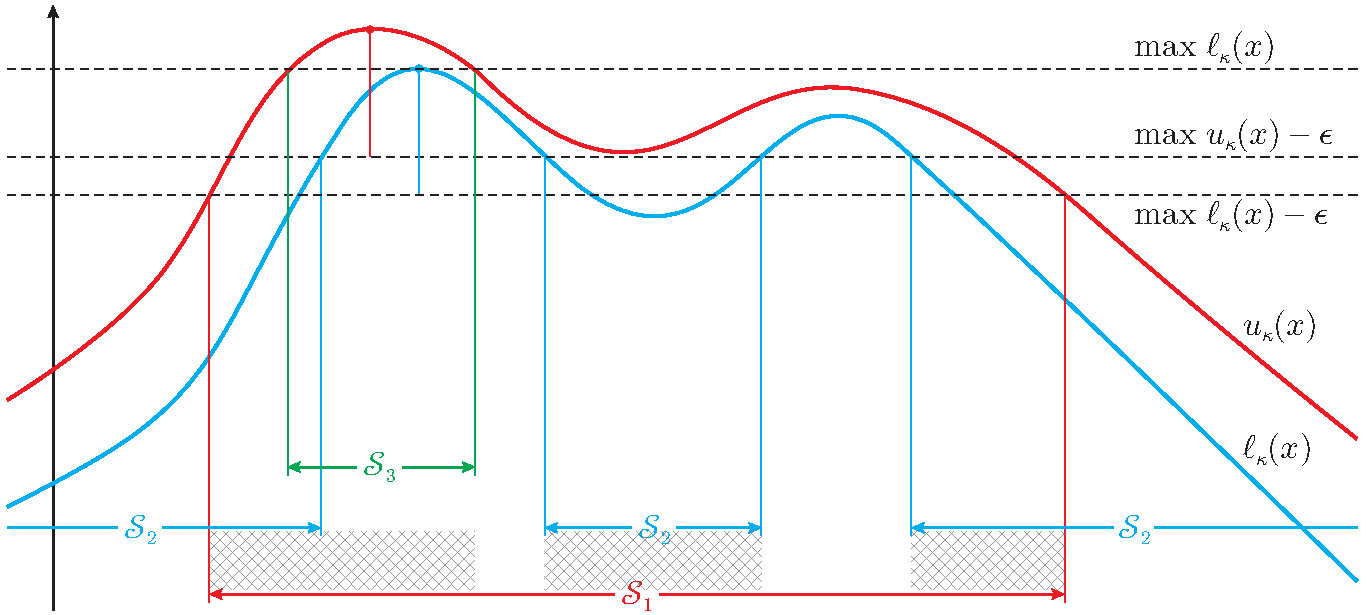
\includegraphics[width=\textwidth]{figures/cb_eps}
  \caption{A one-dimensional example showing the three sets $\mathcal{S}_1$,
           $\mathcal{S}_2$ and $\mathcal{S}_3$, as well as
           the (shaded) confidence region
           $\mathcal{S} = \mathcal{S}_1\cap\mathcal{S}_2\cup\mathcal{S}_3$.}
  \label{fig:cbe}
\end{figure}

\section{Experiments}

\todo{Talk about Hausdorff here?}

\todo{Properly choosing kernel}

\subsection{Synthetic data}

\subsection{Seismographic data}

\bibliographystyle{plain}
\bibliography{report}

\end{document}
